A test was performed to find the fiber length that optimizes the tritium detection efficiency. Two different lengths of scintillating fibers were considered in this study, $1~\meter$ and $20~\cm$ and two different tritium source activity were used, $0.5~\kilo\becquerel/\liter$ and $2.5~\kilo\becquerel/\liter$. As detected tritium decays are proportional to the active area, 5 detectors were simulated for the case of a $0.20~\meter$ fiber length to have the same active area. As the active area of the detector is related to its tritium detection efficiency, the advantage to use long fibers is their large active areas with a small number of cells, reducing the number of photosensors and, consequently, the price of the TRITIUM monitor. However, a smaller length of scintillating fibers reduce de photon absortion produced in the fibers, increasing the tritium detection efficiency per active area.

To find the scintillating fiber length that optimize the tritium detection efficiency, the Tritium-Aveiro prototype, consisting of a similar design as the TRITIUM-IFIC 2 prototype but with $360$ scintillating fibers of $2~\mm$ diameter, was simulated. All optical properties were included in this study in which the photon propagation was included.

The propagation of photons in scintillating fibers was studied. The number of photons produced in a scintillating fiber per tritium electron was compared between all electrons that reach the scintillating fiber and only those the photons of which are detected in time coincidence by the photosensors, shown in Figure \ref{fig:PhotonsFibersYesNoPhotosensors}. Tritium events that produce a high number of photons are mostly detected but the events that produce few photons are seldom detected, resulting in a peak centred at around $25$ photons.  

\begin{figure}[h]
\centering
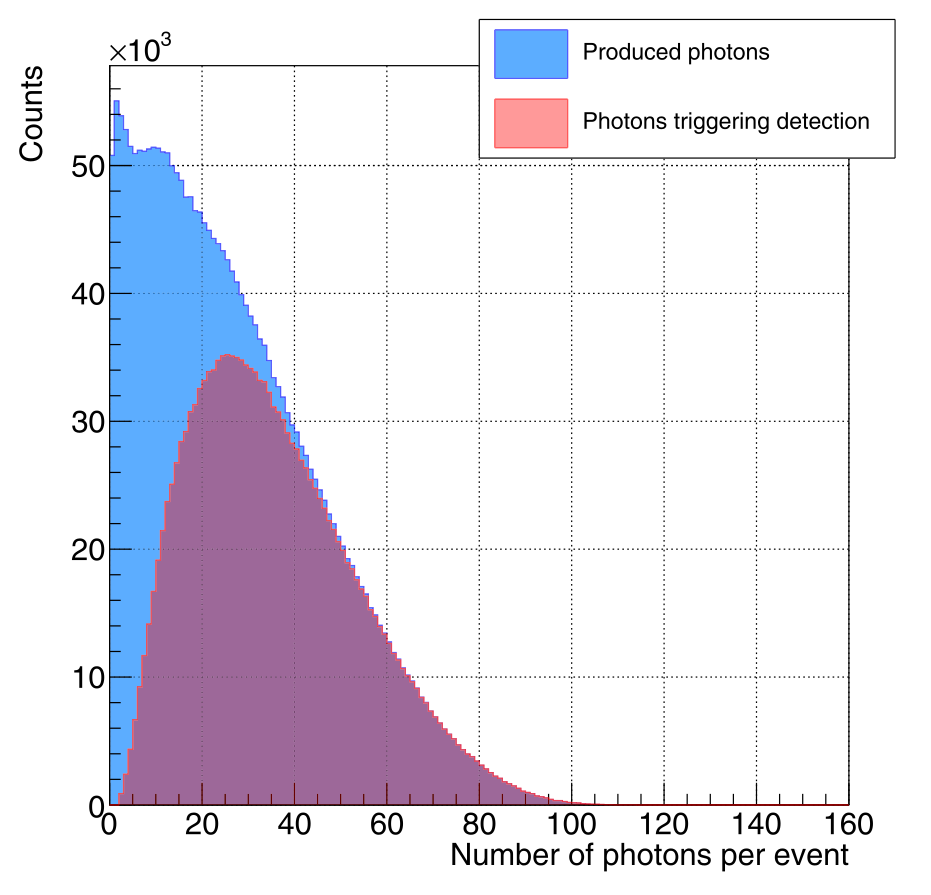
\includegraphics[scale=0.3]{Figures/8SimulationsResults/81TRITIUMDesign/813Length/CollectionPhotonsInFibers.png}
\caption{Number of photons produced in the fiber per tritium event for all tritium events that reach the fiber (blue histogram) and only for tritium events the photons of which are detected by photosensors (red histogram) \cite{SimulationPaperCarlos}.\label{fig:PhotonsFibersYesNoPhotosensors}}
\end{figure}

%Regarding the fiber length study, 

The counts, integred over $60~\min$ and taken over a week, are shown in Figure \ref{fig:CountsOver60minDifferentLength} as a function of the time for both tritium activities and fiber lengths mentioned above. A $25\%$ larger signal is seen for the shorter fiber length in both cases, due principally to the lower absortion of photons in shorter scintillating fibers and the leakage of some photons due to partial photon collection in the fiber. In addition, non simulation effects like the dirty or mechanical imperfections of scintillating fibers increase accentuate this effect.

\begin{figure}[h]
\centering
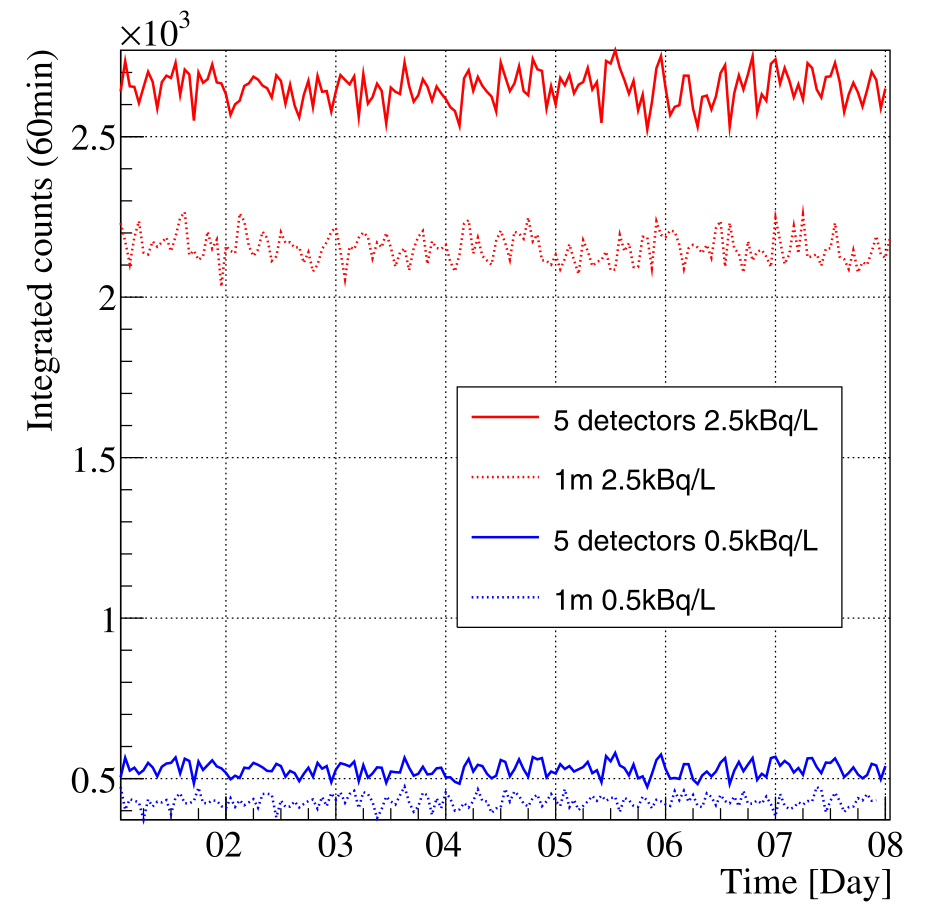
\includegraphics[scale=0.3]{Figures/8SimulationsResults/81TRITIUMDesign/813Length/2DifferentLength.png}
\caption{Simulations of counts integred over $60~\min$, normalized to the same active area and taken over a week for a fiber length of $1~\meter$, dashed lines, and $20~\cm$, solid lines and two different activities, $0.5~\kilo\becquerel/\liter$, blue lines, and $2.5~\kilo\becquerel/\liter$, red lines \cite{SimulationPaperCarlos}. \label{fig:CountsOver60minDifferentLength}}
\end{figure}

